\selectlanguage{italian}%

\section{Soluzione}

Si far� riferimento agli esercizi del capitolo \ref{minimizzazione},
definiti in file di formato \emph{blif }per la minimizzazione ed il
mapping tecnologico mediante SIS.

\subsection{Descrizione in file blif}

Di seguito verrano elencati i relativi file blif, con i quali � possibili
minizzare automaticamente le funzioni sopra descritte.

\label{blif_minimizzazione}

\noindent\begin{minipage}[t]{1\columnwidth}%
In riferimento a \ref{subsec:min1}

\lstinputlisting{esercizio02/listing/blif/esercizio1.blif}%
\end{minipage}

\noindent\begin{minipage}[t]{1\columnwidth}%
In riferimento a \ref{subsec:min2}

\lstinputlisting{esercizio02/listing/blif/esercizio2.blif}%
\end{minipage}

\noindent\begin{minipage}[t]{1\columnwidth}%
In riferimento a \ref{subsec:min3}

\lstinputlisting{esercizio02/listing/blif/esercizio3.blif}%
\end{minipage}

\noindent\begin{minipage}[t]{1\columnwidth}%
In riferimento a \ref{subsec:min4}

\lstinputlisting{esercizio02/listing/blif/esercizio4.blif}%
\end{minipage}

\subsection{Esercizio 1}

La minimizzazione automatica restituisce lo stesso risultato di quella
eseguita manualmente attraverso il comando \emph{full\_simplify}.
Effettuando due diversi tipi di mapping, i valori di area e ritardo
variano secondo le esigenze esposte.\medskip{}

\noindent\begin{minipage}[t]{1\columnwidth}%
\centering

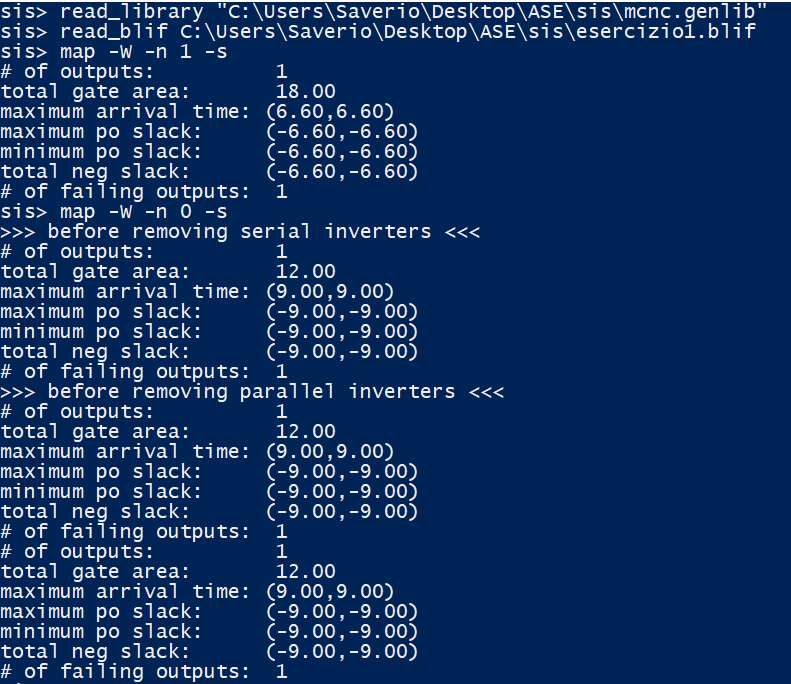
\includegraphics[scale=0.6]{esercizio02/images/minimizzazione1.PNG}

\medskip{}
%
\end{minipage} \noindent Ci� � possibile perch� la libreria � fornita di diversi
componenti, ma se la riduciamo ad un set funzionalmente completo,
\textbf{And} e \textbf{Not} ad esempio, i risultati non variano.

\medskip{}

\noindent\begin{minipage}[t][1\totalheight][c]{1\columnwidth}%
\centering

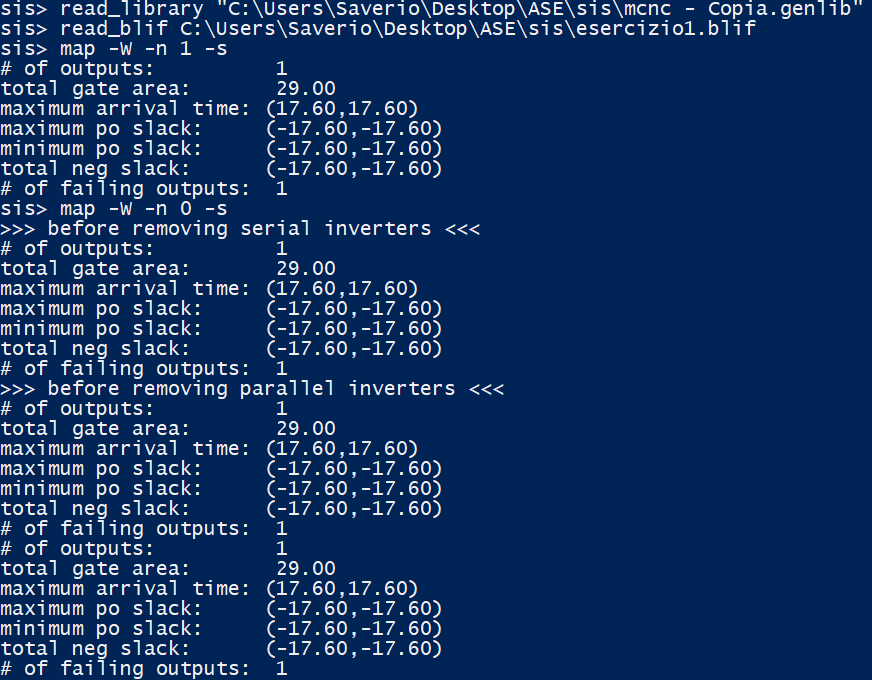
\includegraphics[scale=0.6]{esercizio02/images/minimizzazione1_2.PNG}

\medskip{}
%
\end{minipage}

\subsection{Esercizio 2}

Vogliamo mettere in evidenza in questo esempio come la tecnologia
impatta sulle prestazioni di una rete combinatoria.

\smallskip

\noindent\begin{minipage}[t]{1\columnwidth}%
\centering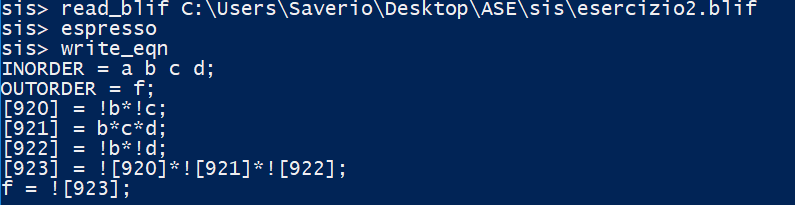
\includegraphics{esercizio02/images/minimizzazione2espresso.PNG}

\medskip{}
%
\end{minipage}

\noindent Utilizzando \emph{espresso} ritroviamo la medesima minimizzazione
attuata manualmente col metodo di Quine Mc Cluskey. I costi della
rete, in termini di numero di litterali $Cl$, numero di ingressi
$Ci$, numero di porte $Cp$ , sono $Cl=7$\foreignlanguage{english}{;
$Ci=10$; $Cp=4$}. Vediamo come si comporta invece la rete con l'
utilizzo della libreria \emph{mcnc}. Ottimizzando l'area occupata:

\medskip{}

\noindent\begin{minipage}[t]{1\columnwidth}%
\centering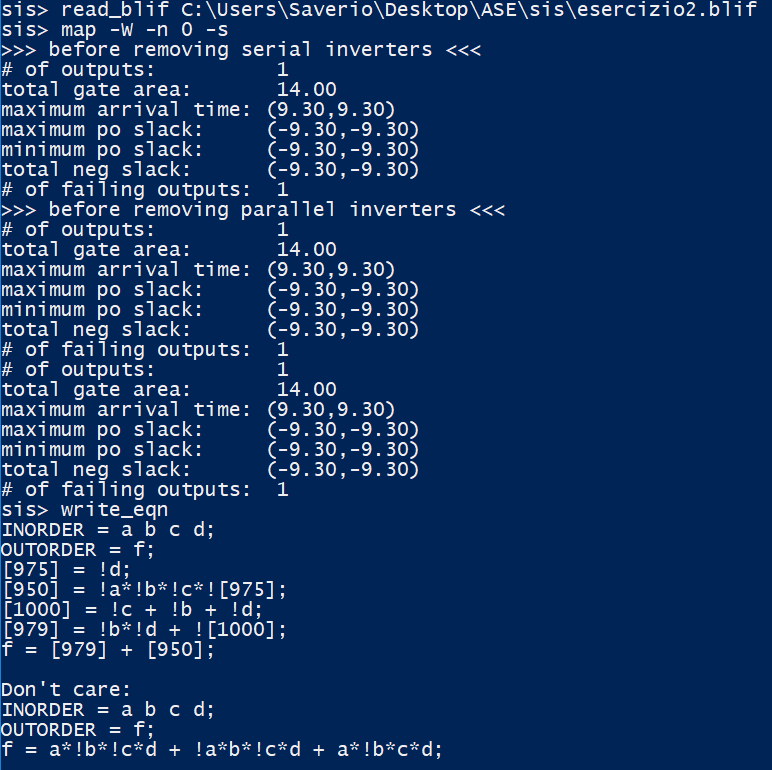
\includegraphics[scale=0.6]{esercizio02/images/minimizzazione2m0.PNG}

\medskip{}
%
\end{minipage}

\noindent In questo caso i costi sono $Cl=9-Ci=13-Cp=5$. I costi
aumentano perch� SIS cerca di usare porte che occupano meno spazio,
non curandosi dei tempi di commutazione e di propagazione dell'informazione
lungo il path critico.

Ottimizzando il ritardo:

\medskip{}

\noindent\begin{minipage}[t]{1\columnwidth}%
\centering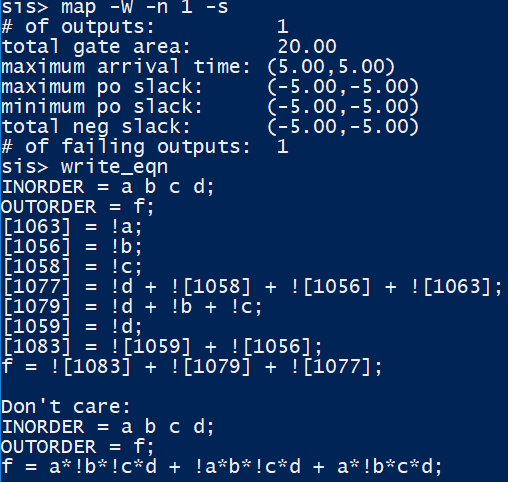
\includegraphics{esercizio02/images/minimizzazione2m1.PNG}

\medskip{}
%
\end{minipage}

\noindent Rilassando il vincolo di area ottieniamo prestazioni vicine
a quelle di \emph{espresso:} $Cl=9$; $Ci=12$; $Cp=4$. Ci� � possibile
perch� la libreria ha a disposizione un adeguato numero di componenti
da utilizzare, situazione non sempre veritiera.

\newpage

\subsection{Esercizio 4}

Proviamo ad applicare il rugged-script ad un rete multi-uscita:

\medskip{}

\noindent\begin{minipage}[t]{1\textwidth}%
\centering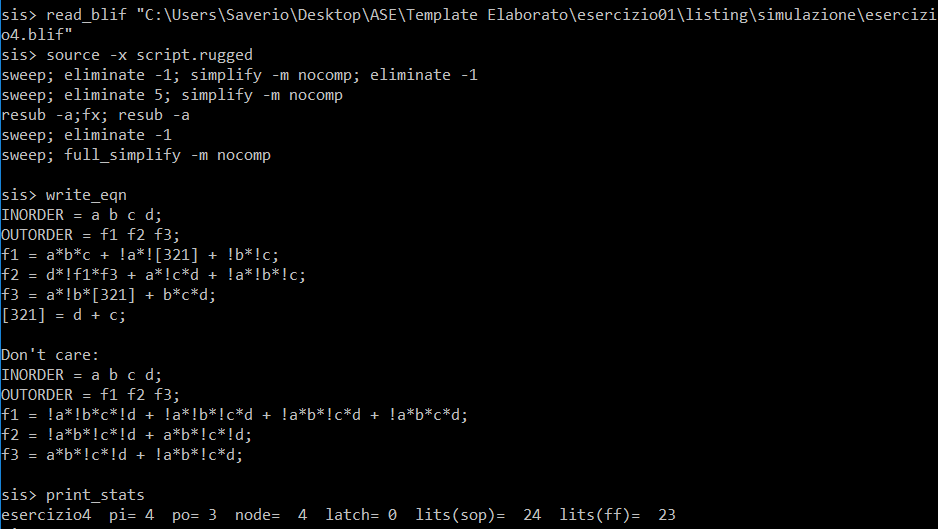
\includegraphics[width=17.5cm]{esercizio02/images/minimizzazione3ruggedscript.PNG}

\medskip{}
%
\end{minipage}

\noindent La minimizzazione sub-ottima ottenuta con questo metodo
euristico � simile a quella ricavata da Mc Cluskey multi-funzione,
a conferma del fatto che il rugged-script si rivela una buona sequenza
per le trasformazioni da applicare alla rete. Rimappiamo la nostra
rete su un fpga avente componenti elementari a quattro ingressi.

\medskip{}

\noindent\begin{minipage}[t]{1\textwidth}%
\centering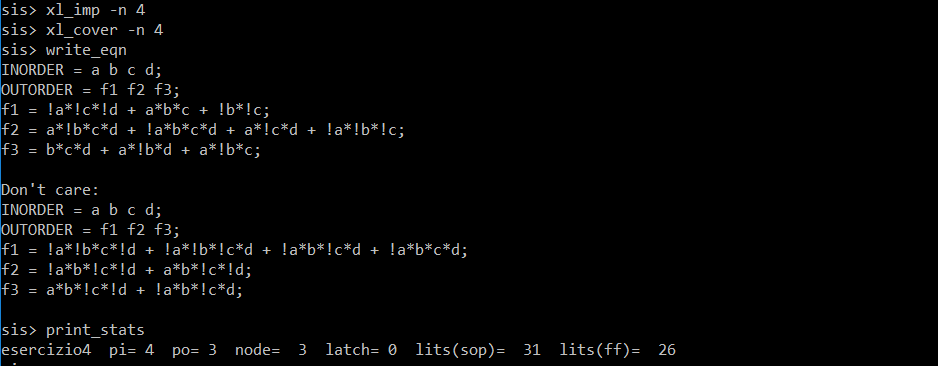
\includegraphics[width=17.5cm]{esercizio02/images/minimizzazione3sureteaquattrolivelli.PNG}

\medskip{}
%
\end{minipage}

\noindent Il mapping � stato possibile perch� il fan-in dei nodi
della rete non � maggiore del numero di input di una cella. Al seguito
di questa verifica, � stata effettuata la minimizzazione del numero
di nodi della rete e l'associazione di questi alle celle Xilinx. Il
numero di nodi utilizzati per sintetizzare la rete � diminuito e il
numero di letterali � aumentato di 7 unit�: un nodo � stato eliminato
sostituendo la sua espressione nei nodi a valle. Ci� ha consentito
un risparmio di area, in termini di celle, ed eventualmente anche
di tempo, grazie ad una dipendenza pi� diretta dei nodi a valle dagli
input primari. \selectlanguage{italian}%

